\documentclass{assignment}
\UsingEnglish
\ProjectInfos*{Introduction to System System}{EE140}{Fall, 2020}{Assignment 2}{Due time : 10:15, Sept 25, 2020 (Friday)}{陈稼霖}{45875852}
\begin{document}
\begin{prob}[Conditional probability, 10 pts]
    Given a binary communication channel where $A=$input and $B=$output, let $P(A)=0.3$, $P(B\vert A)=0.8$, and $P(\bar{B}\vert\bar{A})=0.6$. Find $P(A\vert B)$ and $P(\bar{A}\vert\bar{B})$.
\end{prob}
\begin{sol}
    Using the law of total probability, the probability of getting output $B$ is
    \begin{align}
        \notag P(B)=&P(B\vert A)P(A)+P(B\vert\bar{A})P(\bar{A})=P(B\vert A)P(A)+[1-P(\bar{B}\vert\bar{A})][1-P(A)]\\
        =&0.8\times 0.3+(1-0.6)\times(1-0.3)=0.52.
    \end{align}
    Using Bayes' theorem, we have
    \begin{align}
        P(A\vert B)=\frac{P(B\vert A)P(A)}{P(B)}=\frac{0.8\times 0.3}{0.52}=\frac{6}{13},
    \end{align}
    and
    \begin{align}
        P(\bar{A}\vert\bar{B})=\frac{P(\bar{B}\vert\bar{A})P(\bar{A})}{P(\bar{B})}=\frac{P(\bar{B}\vert\bar{A})[1-P(A)]}{P(\bar{B})}=\frac{0.6\times(1-0.3)}{1-0.52}=\frac{7}{8}.
    \end{align}
\end{sol}


\begin{prob}[Property of PDF, 20pts]
    The joint pdf of random variables $X$ and $Y$ is $f(x,y)=Axye^{-2(x+y)}$, $x\geq 0$, $y\geq 0$. Find the following.
    \begin{itemize}
        \item[1)] Find the constant $A$.
        \item[2)] Find the marginal pdfs of $X$ and $Y$, $f_X(x)$ and $f_Y(y)$.
        \item[3)] Are $X$ and $Y$ statistically independent? Justify your answer.
        \item[4)] Find the probability density function of $Z=X+Y$.
    \end{itemize}
\end{prob}
\begin{sol}
    \begin{itemize}
        \item[1)] As a property of pdf,
        \begin{align}
            \notag\int_0^{+\infty}\int_0^{+\infty}f(x,y)\,dx\,dy=&\int_0^{+\infty}\int_0^{+\infty}Axye^{-2(x+y)}\,dx\,dy=A\left[\int_0^{+\infty}xe^{-2x}\,dx\right]\left[\int_0^{+\infty}ye^{-2y}\,dy\right]\\
            \notag=&A\left[\int_0^{+\infty}xe^{-2x}\,dx\right]^2=A\left[-\frac{1}{2}\int_0^{+\infty}xd\left(e^{-2x}\right)\right]^2\\
            \notag=&A\left[\left.-\frac{1}{2}\left(xe^{-2x}\right)\right\rvert_0^{+\infty}+\frac{1}{2}\int_0^{+\infty}e^{-2x}\,dx\right]^2\\
            \notag=&A\left[\frac{1}{4}\right]^2=\frac{A}{16}=1,
        \end{align}
        which gives us that
        \begin{align}
            A=16.
        \end{align}
        \item[2)] The marginal pdf of $X$ is
        \begin{align}
            \notag f_X(x)=&\int_{-\infty}^{+\infty}f(x,\beta)\,d\beta=\int_{-\infty}^{+\infty}16x\beta e^{-2(x+\beta)}\,d\beta\\
            \notag=&16xe^{-2x}\int_{-\infty}^{+\infty}\beta e^{-2\beta}\,d\beta\\
            =&4xe^{-2x},
        \end{align}
        and similarly, the marginal pdf of $Y$ is
        \begin{align}
            \notag f_Y(y)=&\int_{-\infty}^{+\infty}f(\alpha,y)\,d\alpha=\int_{-\infty}^{+\infty}16\alpha ye^{-2(\alpha+y)}\,d\alpha=4ye^{-2y}.
        \end{align}
        \item[3)] \textbf{$X$ and $Y$ are statistically independent}, since
        \begin{align}
            f(x,y)=16xye^{-2(x+y)}=\left(4xe^{-2x}\right)\left(4ye^{-2y}\right)=f_X(x)f_Y(y),\qquad\text{for all }x\geq 0,y\geq 0.
        \end{align}
        \item[4)] Since $X$ and $Y$ are independent, the pdf of $Z=X+Y$ is the convolution of pdfs of $X$ and $Y$:
        \begin{align}
            \notag f_Z(z)=&\int_0^zf_X(z-u)f_Y(u)\,du\\
            \notag=&\int_0^z4(z-u)e^{-2(z-u)}\cdot 4ue^{-2u}\,du\\
            \notag=&16e^{-2z}\int_0^z(z-u)u\,du\\
            =&\frac{8}{3}z^3e^{-2z}.
        \end{align}
    \end{itemize}
\end{sol}

\begin{prob}[Gaussian random variables, 20pts]
    Assume two random variables $X$ and $Y$ are jointly Gaussian with mean $m_x=1$, $m_y=2$, and variances $\sigma_x^2=1$, $\sigma_y^2=4$.
    \begin{itemize}
        \item[1)] Write down the expressions for their marginal pdfs.
        \item[2)] Assume the correlation coefficient is $\rho_{XY}=0.5$, a new random variables is defined as $Z=X+Y$, find the expression for the pdf of $Z$.
        \item[3)] Express the following probabilities using the $Q$ function.
        \begin{itemize}
            \item[a)] $P(\abs{X}\leq 5)$
            \item[b)] $P(-2<Y\leq 12)$
        \end{itemize}
    \end{itemize}
\end{prob}
\begin{sol}
    \begin{itemize}
        \item[1)] The expression for marginal pdf of $X$ is
        \begin{align}
            f_X(x)=\frac{1}{\sqrt{2\pi\sigma_x^2}}\exp\left[-\frac{1}{2\sigma_x^2}(x-m_x)^2\right]=\frac{1}{\sqrt{2\pi}}\exp\left[-\frac{1}{2}(x-1)^2\right],
        \end{align}
        and the expression for marginal pdf of $Y$ is
        \begin{align}
            f_Y(y)=\frac{1}{\sqrt{2\pi\sigma_y^2}}\exp\left[-\frac{1}{2\sigma_y^2}(y-m_y)^2\right]=\frac{1}{\sqrt{2\pi\cdot 4}}\exp\left[-\frac{1}{2\times 4}(y-2)^2\right].
        \end{align}
        \item[2)] The jointly pdf of $X$ and $Y$ is
        \begin{align}
            \notag f_{XY}(x,y)=&\frac{1}{2\pi\sigma_x\sigma_y\sqrt{1-\rho_{XY}^2}}\exp\left\{-\frac{1}{2(1-\rho_{XY}^2)}\left[\frac{(x-m_x)^2}{\sigma_x^2}-\frac{2\rho(x-m_x)(y-m_y)}{\sigma_x\sigma_y}+\frac{(y-m_y)^2}{\sigma_y^2}\right]\right\}\\
            =&\frac{1}{2\pi\sqrt{3}}\exp\left\{-\frac{1}{2\times\frac{3}{4}}\left[(x-1)^2-\frac{(x-1)(y-2)}{2}+\frac{(y-2)^2}{4}\right]\right\}.
        \end{align}
        The expression of the pdf of $Z$ is
        \begin{align}
            \notag f_Z(z)=&\int_{-\infty}^{+\infty}f_{XY}(u,z-u)\,du\\
            \notag=&\int_{-\infty}^{+\infty}\frac{1}{2\pi\sqrt{3}}\exp\left\{-\frac{1}{2\times\frac{3}{4}}\left[(u-1)^2-\frac{(u-1)(z-u-2)}{2}+\frac{(z-u-2)^2}{4}\right]\right\}\,du\\
            \notag=&\int_{-\infty}^{+\infty}\frac{1}{\sqrt{2\pi\cdot 7}}\frac{1}{\sqrt{2\pi\frac{3}{7}}}\exp\left\{-\frac{1}{2\times\frac{3}{7}}\left[(u-\frac{2}{7}(z+\frac{1}{2}))^2+\frac{3}{49}(z-3)^2\right]\right\}\\
            =&\frac{1}{\sqrt{2\pi 7}}\exp\left\{-\frac{1}{14}(z-3)^2\right\}.
        \end{align}
        \item[3)] 
        \begin{itemize}
            \item[a)] 
            \begin{align}
                \notag P(\abs{X}\leq 5)=&P(-5\leq X\leq 5)=1-P(X>5)-P(X<-5)=1-P(X>5)-P(X>7)\\
                =&1-Q(5-1)-Q(7-1)=1-Q(4)-Q(6).
            \end{align}
            \item[b)] 
            \begin{align}
                \notag P(-2<Y\leq 12)=&1-P(Y>12)-P(Y<-2)=1-P(Y>12)-P(Y>6)\\
                =&1-Q\left(\frac{12-2}{2}\right)-P\left(\frac{6-2}{2}\right)=1-Q(5)-Q(2).
            \end{align}
        \end{itemize}
    \end{itemize}
\end{sol}

\begin{prob}[Random Process: probability, 20pts]
    A fair die is thrown. Depending on the number of spots on the up face, the following random process are generated.
    \begin{itemize}
        \item[1)] Sketch several examples of sample functions of each case. ($A>0$ is a constant).
        \begin{itemize}
            \item[a)] $X(t,\zeta)=\left\{\begin{array}{ll}
                2A,&1\text{ or }2\text{ spots up}\\
                0,&3\text{ or }4\text{ spots up}\\
                -2A,&5\text{ or }6\text{ spots up}
            \end{array}\right.$
            \item[b)] $X(t,\zeta)=\left\{\begin{array}{ll}
                2A,&1\text{ or }2\text{ spots up}\\
                At,&3\text{ or }4\text{ spots up}\\
                -At,&5\text{ or }6\text{ spots up}
            \end{array}\right.$
        \end{itemize}
        \item[2)] What are the following probabilities for each case (case a and case b in 1))?
        \begin{itemize}
            \item[i.] $P(X(4)\geq A)$ ($X(4)$ means $X(t=4,\zeta)$, which is a random variable.)
            \item[ii.] $P(X(2)\leq 0)$ ($X(2)$ means $X(t=2,\zeta)$, which is a random variable.)
        \end{itemize}
    \end{itemize}
\end{prob}
\begin{sol}
    \begin{itemize}
        \item[1)] 
        \begin{itemize}
            \item[a)] As shown in figure \ref{4-a}.
            \item[b)] As shown in figure \ref{4-b}.
            \begin{figure}[h]
                \centering
                \subfigure[Sample functions of a)]{
                \label{4-a}
                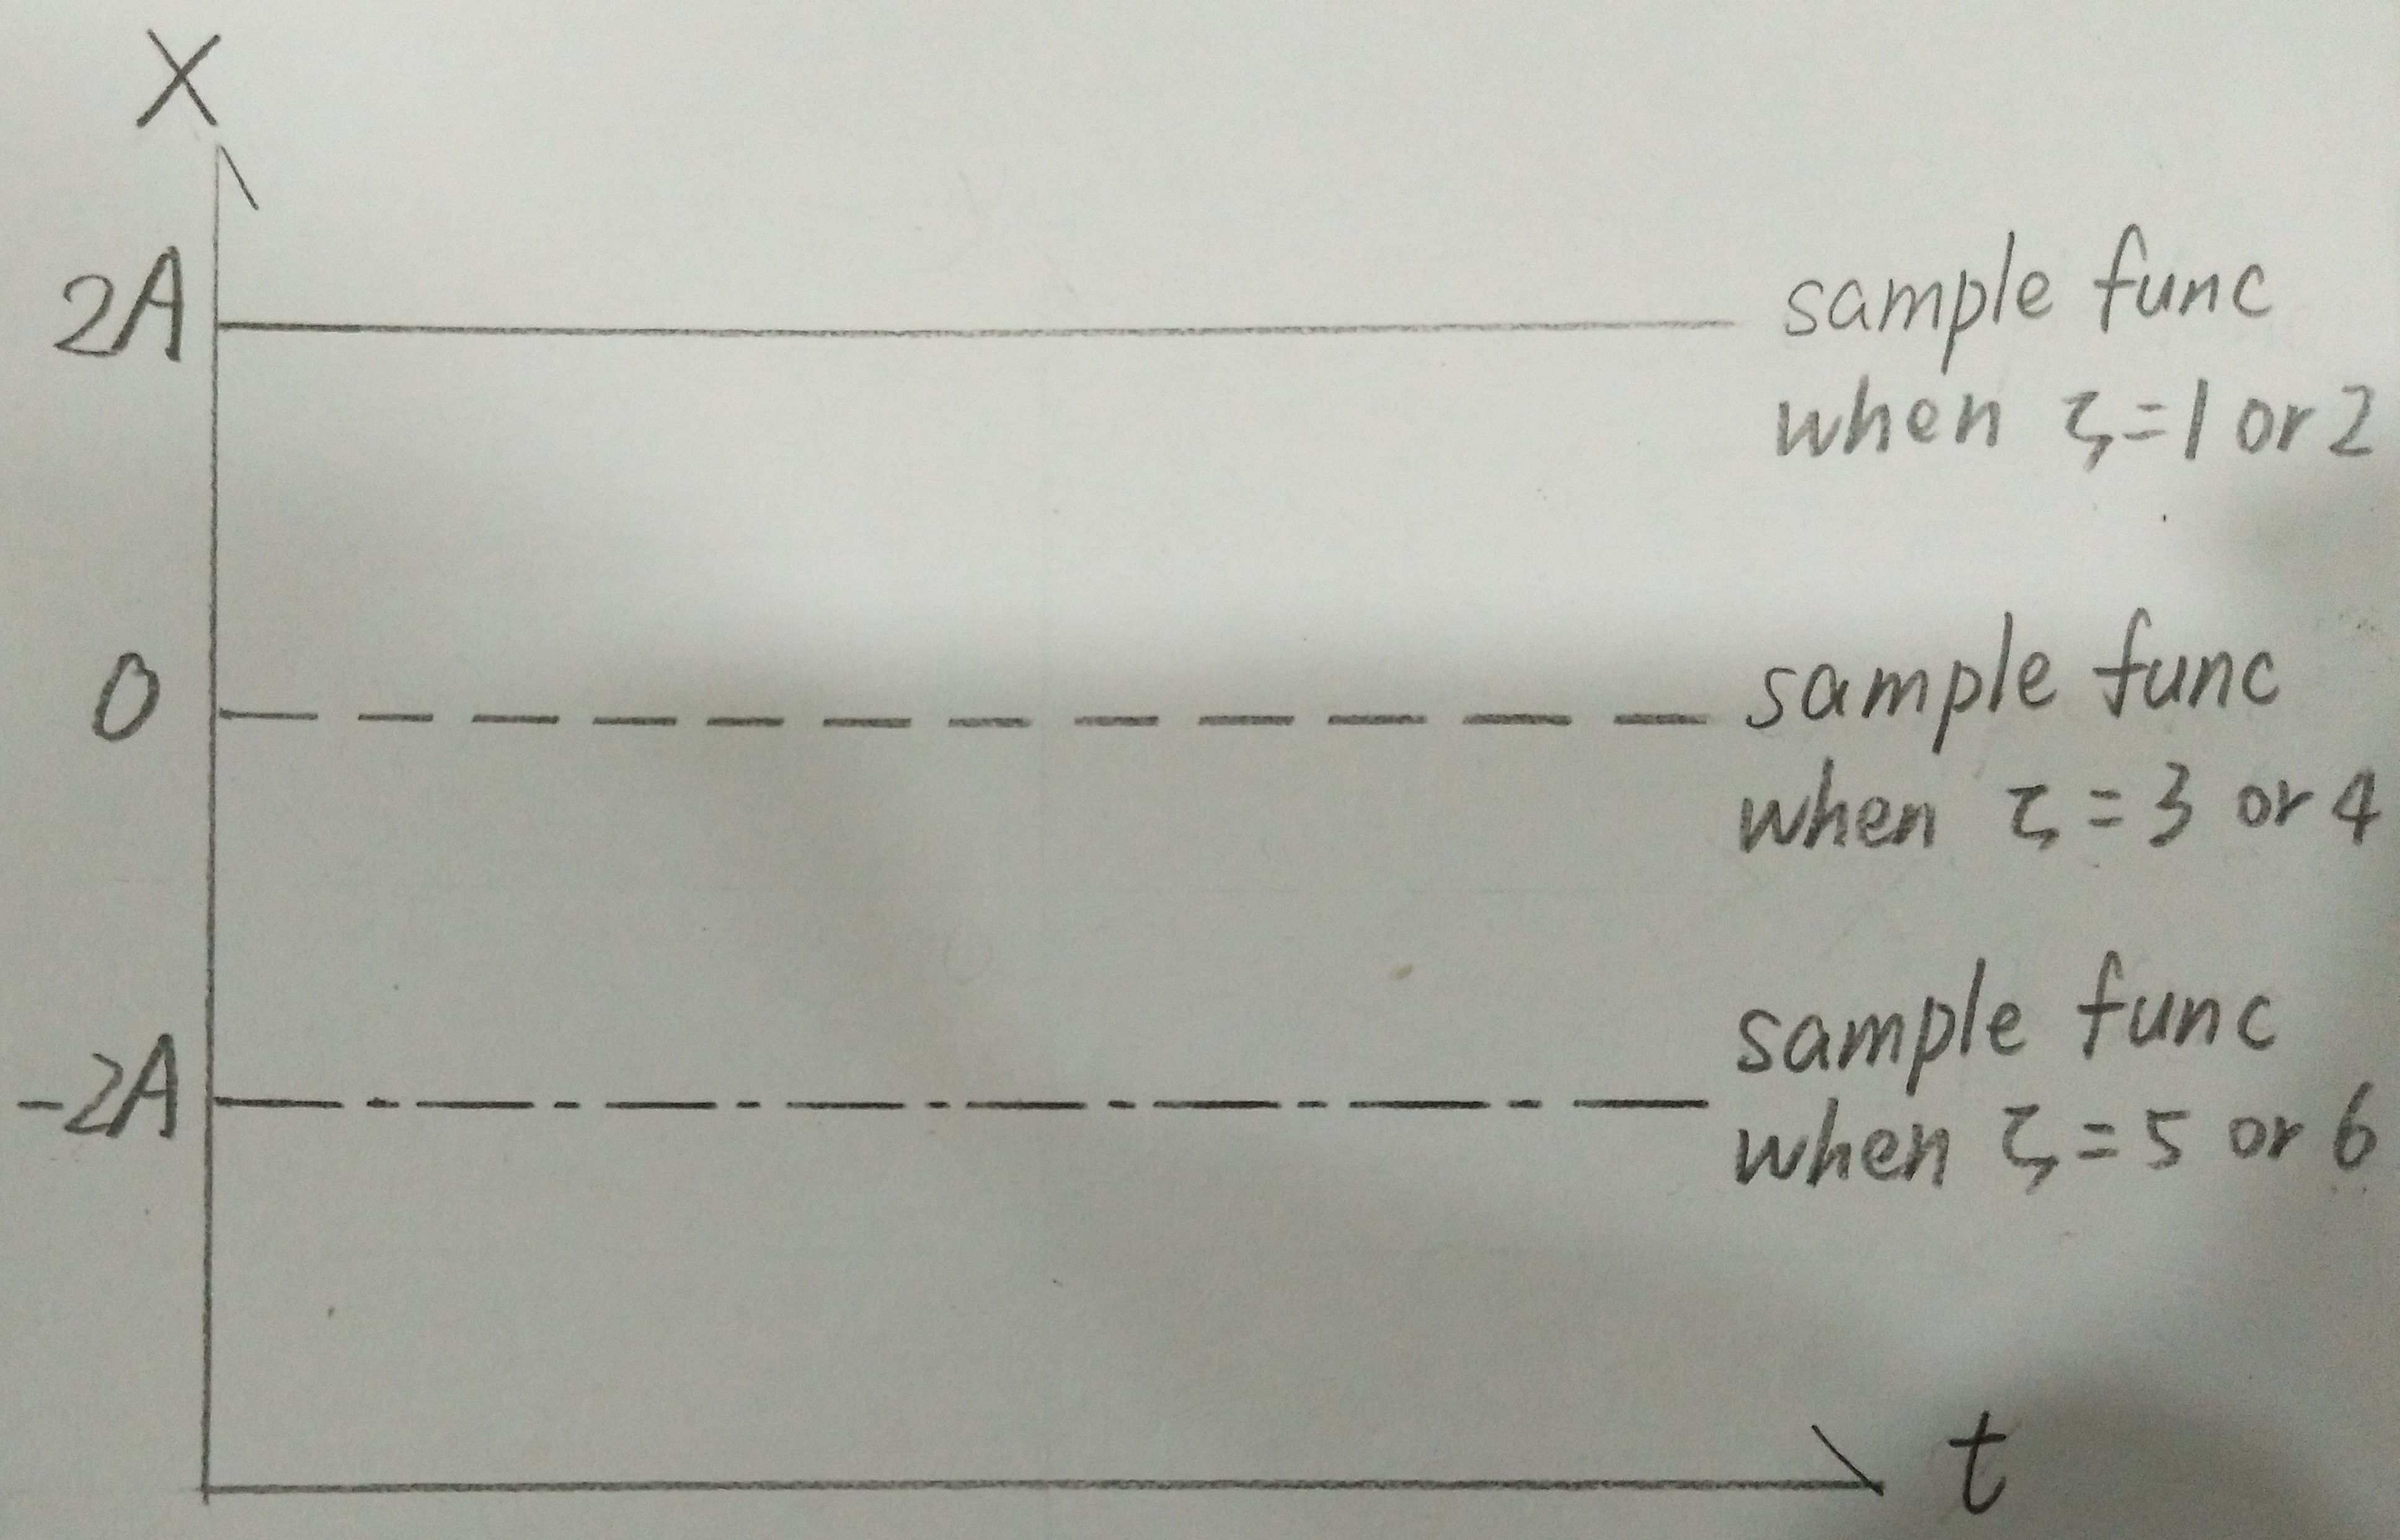
\includegraphics[width=0.45\textwidth]{Assignment-2-Problem-4-a.jpg}}
                \subfigure[Sample functions of b)]{
                \label{4-b}
                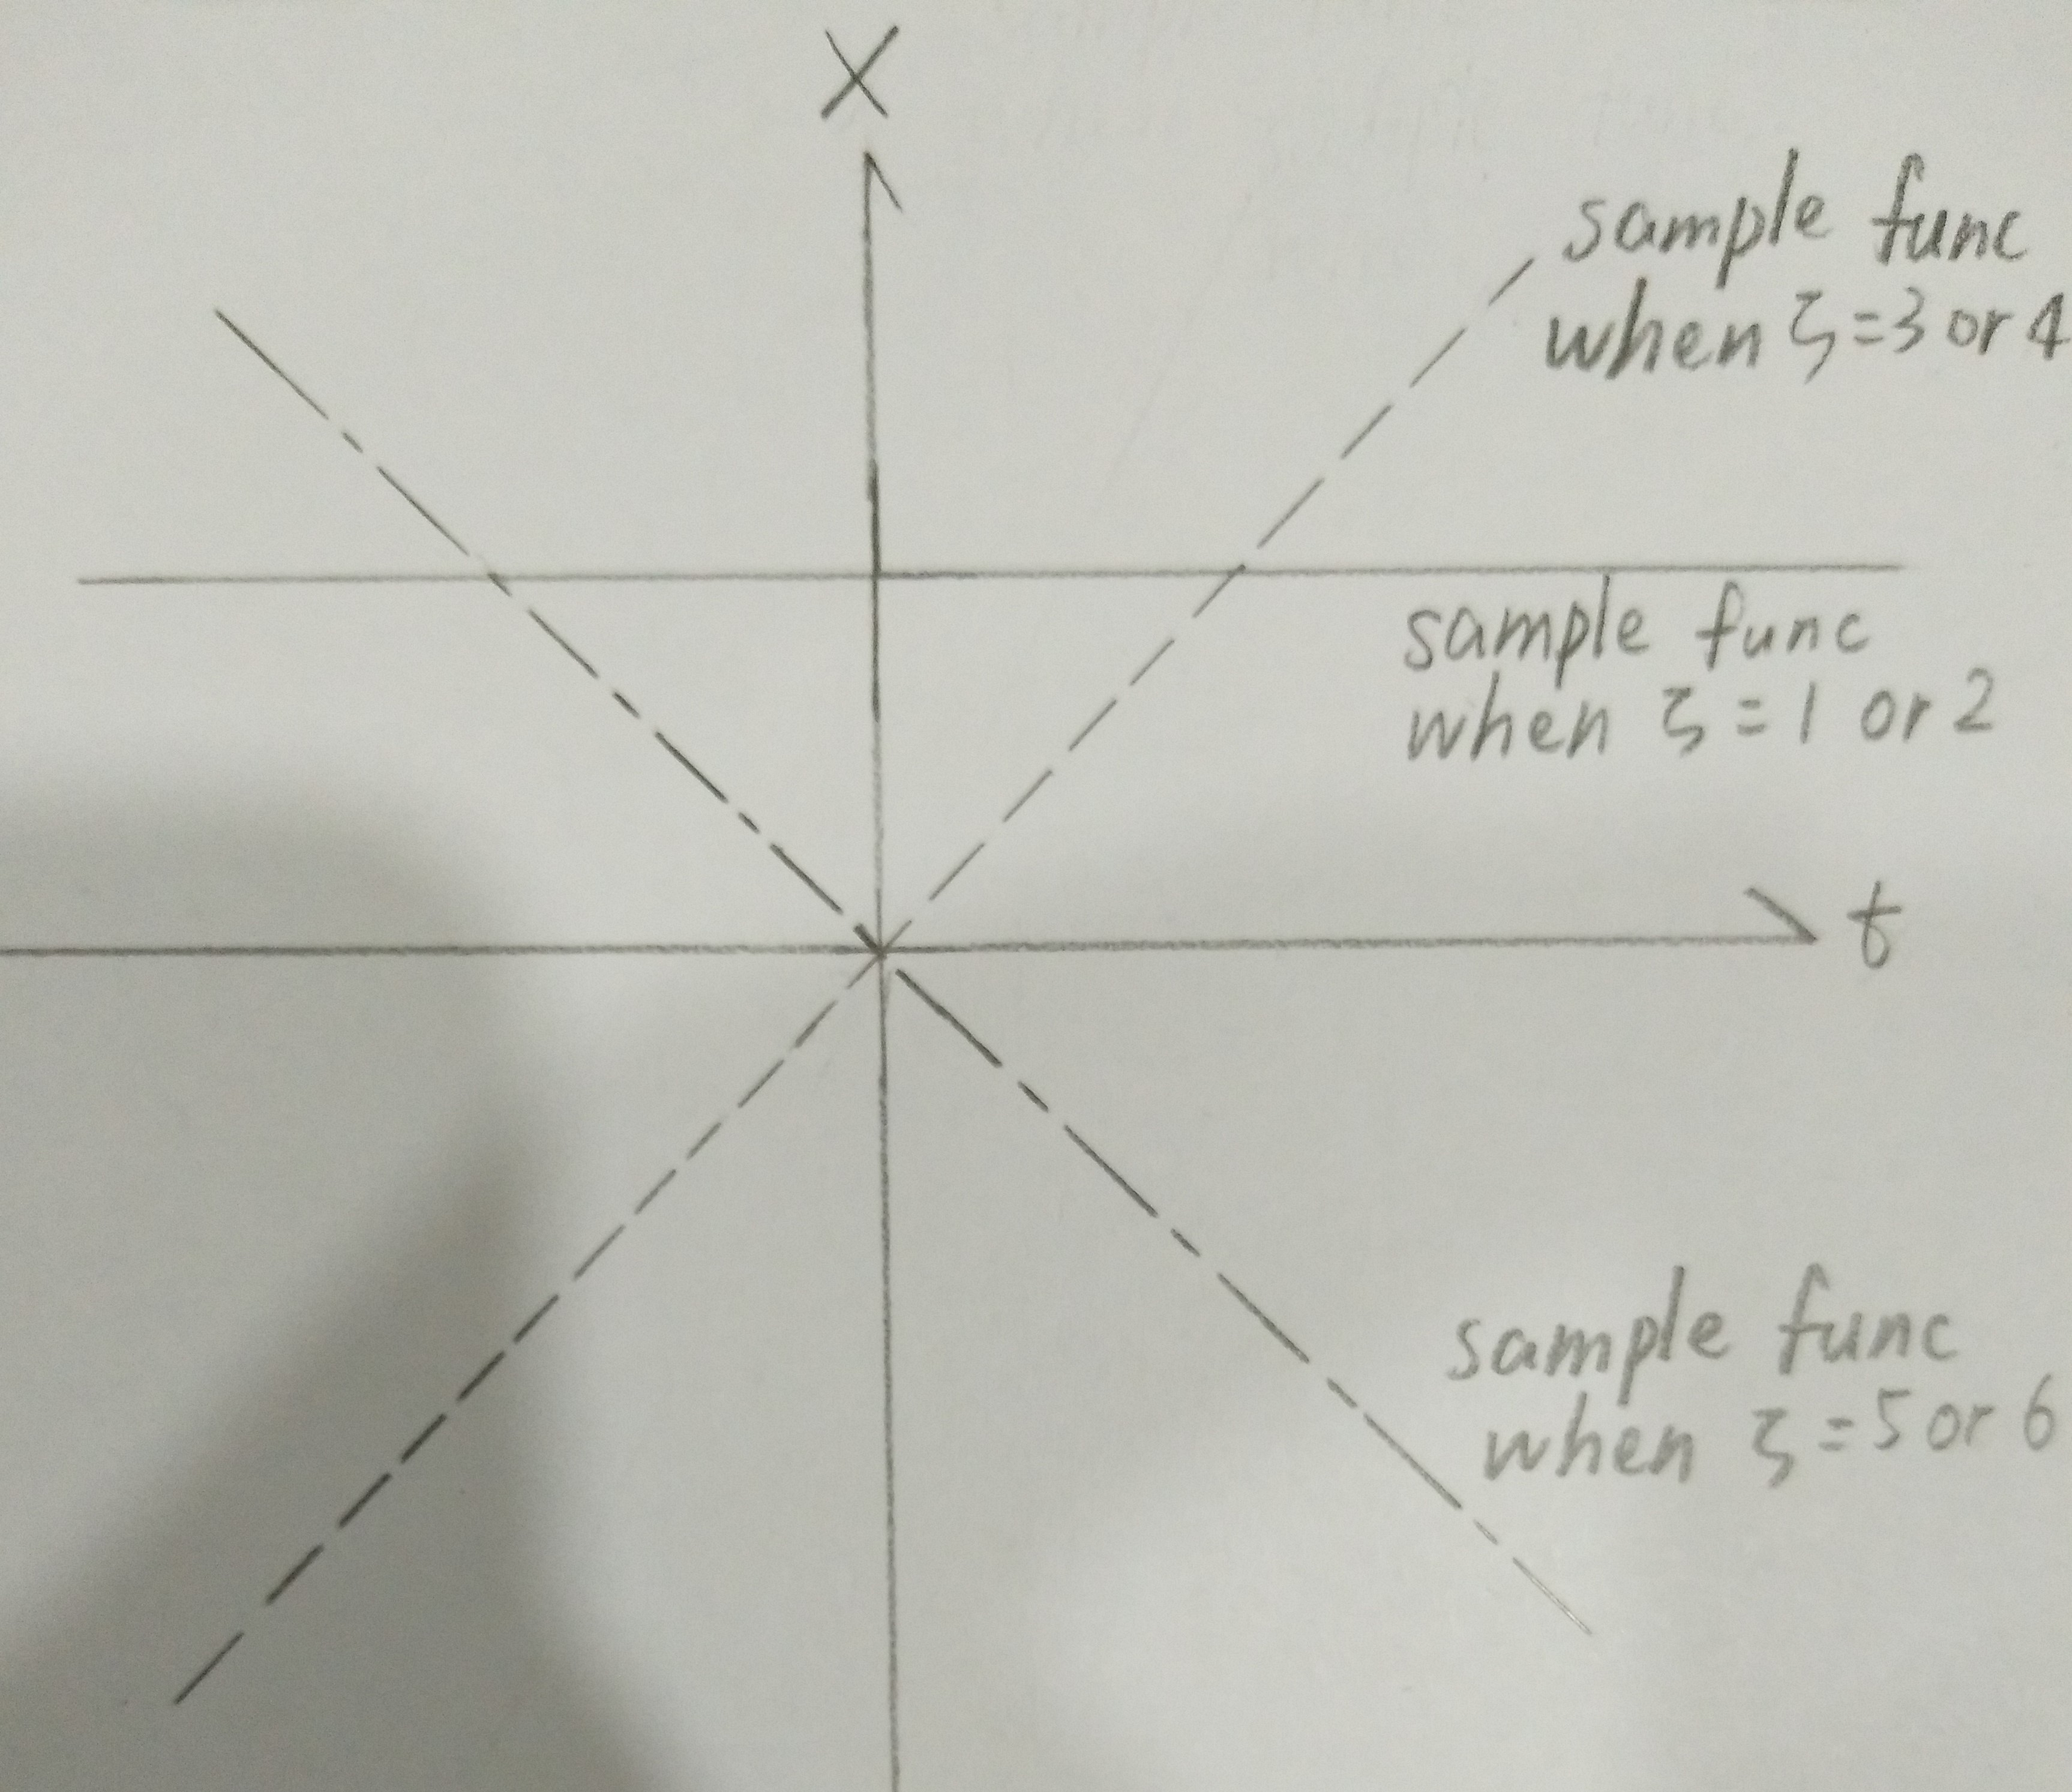
\includegraphics[width=0.45\textwidth]{Assignment-2-Problem-4-b.jpg}}
                \caption{}
                \label{4}
            \end{figure}
        \end{itemize}
        \item[2)] 
        \begin{itemize}
            \item[i.] For case a,
            \begin{align}
                P(X(4)\geq A)=\frac{1}{3}.
            \end{align}
            For case b,
            \begin{align}
                P(X(4)\geq A)=\frac{2}{3}.
            \end{align}
            \item[ii.] For case a,
            \begin{align}
                P(X(2)\leq 0)=\frac{2}{3}.
            \end{align}
            For case b,
            \begin{align}
                P(X(2)\leq 0)=\frac{1}{3}.
            \end{align}
        \end{itemize}
    \end{itemize}
\end{sol}

\begin{prob}[Random Process: mean, variance, autocorrelation, 30 pts]
    Let the sample function of a random process be given by $X(t)=A\cos 2\pi f_0t$, where $f_0$ is fixed and $A$ has the pdf
    \[
        f_A(a)=\frac{1}{\sqrt{2\pi\sigma_a^2}}e^{-\frac{\abs{a-\mu_a}^2}{2\sigma_a^2}}.
    \]
    The mean and variance of $A$ are given by $\mu_a=0$, $\sigma_a^2=4$.
    \begin{itemize}
        \item[1)] Find the mean and variance of random process $X(t)$ at time $t_0$.\\
        (Hint: ensemble-mean; Note that $\cos 2\pi f_0t_0$ is just a constant.)
        \item[2)] Find the autocorrelation function of $X(t)$.
        \item[3)] Is $X(t)$ stationary?
        \item[4)] Find the time average mean and autocorrelation function of $X(t)$.\\
        (Hint1: the time average mean can be calculated as $\langle X(t)\rangle=\lim_{T\rightarrow\infty}\frac{1}{2T}\int_{-T}^Tx(t)\,dt$, the time average autocorrelation function can be calculated as $\langle X(t)X(t+\tau)\rangle=\lim_{T\rightarrow\infty}\frac{1}{2T}\int_{-T}^Tx(t)x(t+\tau)\,dt$\\
        Hint2: For periodic signal, $\langle X(t)\rangle=\frac{1}{T}\int_0^Tx(t)\,dt$, and $\langle X(t)X(t+\tau)\rangle=\frac{1}{T}\int_0^Tx(t)x(t+\tau)\,dt$)
        \item[5)] Is the $X(t)$ ergodic?
    \end{itemize}
\end{prob}
\begin{sol}
    \begin{itemize}
        \item[1)] The mean of random process $X(t)$ at time $t_0$ is
        \begin{align}
            E(X(t_0))=E[X(t=t_0)]=\int_{-\infty}^{+\infty}a\cos(2\pi f_0t_0)\frac{1}{\sqrt{2\pi\sigma_a^2}}e^{-\frac{\abs{a-\mu_a}^2}{2\sigma_a^2}}\,da=0.
        \end{align}
        The variance of random process $X(t)$ at time $t_0$ is
        \begin{align}
            \sigma_X^2(t_0)=E\left[\abs{X(t_0)-\overline{X(t_0)}}^2\right]=E[X(t_0)^2]=E[A^2]\cos^2(2\pi f_0t_0)=\sigma_a^2\cos^2(2\pi f_0t_0)=4\cos^2(2\pi f_0t_0).
        \end{align}
        \item[2)] Let $t_1=t$, $t_2=t+\tau$. The autocorrelation function of $X(t)$ is
        \begin{align}
            \notag R_X(t_1,t_2)=&E[X(t_1)X(t_2)]=X[A\cos(2\pi f_0t)A\cos(2\pi f_0(t+\tau))]\\
            \notag=&E[A^2]\cos(2\pi f_0t)\cos[2\pi f_0(t+\tau)]\\
            \notag=&\sigma_a^2\cos(2\pi f_0t)\cos[2\pi f_0(t+\tau)]\\
            =&4\cos(2\pi f_0t)\cos[2\pi f_0(t+\tau)].
        \end{align}
        \item[3)] \textbf{No}, since the second-order statistics of $X(t)$ does not depend only on the time gap $\tau$, but also on the begin time $t$.
        \item[4)] $X(t)$ is a periodic signal. Its time mean is
        \begin{align}
            \notag\langle X(t)\rangle=&\frac{1}{T}\int_0^Tx(t)\,dt=f_0\int_0^{1/f_0}A\cos(2\pi f_0t)\,dt\\
            =&0.
        \end{align}
        and its autocorrelation function is
        \begin{align}
            \notag\langle X(t)X(t+\tau)\rangle=&\frac{1}{T}\int_0^Tx(t)x(t+\tau)\,dt=f_0\int_0^{1/f_0}A\cos(2\pi f_0t)A\cos(2\pi f_0(t+\tau))\,dt\\
            \notag=&A^2f_0\frac{1}{2}\int_0^{1/f_0}\cos[2\pi f_0(2t+\tau)]+\cos[2\pi f_0\tau]\,dt\\
            =&\frac{A^2}{2}\cos(2\pi f_0\tau).
        \end{align}
        \item[5)] \textbf{Yes}, since the ensemble average equals the time average.
    \end{itemize}
\end{sol}
\end{document}